\documentclass[sigconf]{acmart}

\usepackage{hyperref}

%\usepackage{endfloat}
%\renewcommand{\efloatseparator}{\mbox{}} % no new page between figures

\usepackage{booktabs} % For formal tables

\settopmatter{printacmref=false} % Removes citation information below abstract
\renewcommand\footnotetextcopyrightpermission[1]{} % removes footnote with conference information in first column
\pagestyle{plain} % removes running headers


\begin{document}
\title{Natural Language Processing (NLP) to Analyze Human Speech Data}

\author{Ashok Reddy Singam}
\orcid{HID337}
\affiliation{%
  \institution{Indiana University}
  \streetaddress{711 N Park Ave}
  \city{Bloomington} 
  \state{Indiana} 
  \postcode{47408}
}
\email{asingam@iu.edu}

\author{Anil Ravi}
\orcid{HID333}
\affiliation{%
  \institution{Indiana University}
  \streetaddress{711 N Park Ave}
  \city{Bloomington} 
  \state{Indiana} 
  \postcode{47408}
}
\email{anilravi@iu.edu}

\begin{abstract}
Extracting meaningful information from large volumes of unstructured human language and deriving sense out of this information is a challenging \textit{Big Data} application. Processing natural language and converting it into meaningful information is a complex task. For humans, understanding language is so natural. But training computers to perform these tasks is extremely challenging task and has huge implications in many areas of our lives. Automatic speech recognition (ASR) and natural language processing (NLP) based intelligent system can be  used in several human machine interface applications both in consumer and industrial sector. A discussion on describing the architecture, building blocks, performance and applications for such system that would use latest ASR and NLP APIs is covered.
\end{abstract}

\keywords{i523, HID333, HID337, Natural Language Processing, Automatic Speech Recognition, Voic Recognition}

\maketitle

\section{Introduction}
The advancements of digital signal processing, large data processing and natural language processing technologies made speech/voice recognition applications more sophisticated to help solving social and industrial problems. For example, having an intelligent automatic voice recognition system in home to recognize and differentiate between the family members and outsiders would add great value to modern society in terms of assisting in their busy life as well provide necessary help/guidance in offering day-to-day problem solutions, personalized entertainment,  and safety/security. In another example, these systems can provide personalized customer care experience through voice and face recognition by engaging them based on their interests/hobbies. Google home, Alexa, and Siri have become part of the main stream human life activities to seek information and get entertainment by directly speaking with these devices.
\par\null\par
The hypothetical intelligent voice system would need the following technologies to work together:
 \begin{itemize}
     \item Highly efficient voice sensors and high speed digital signal processors.
     \item Automatic Voice Recognition (AVR) hardware and software algorithms.
     \item Machine Learning (ML) algorithms to classify and learn the voice patterns.
     \item Machine learning algorithms to understand family members habits and behaviors.
     \item Natural Language Processing (NLP) algorithms to precisely recognize and process the voice data.
 \end{itemize}
\par\null\par
 Open Source and/or Other tools:
 \begin{itemize}
     \item Google Cloud Speech API or Alexa Voice Service (AVS)
     \item Audio processing hardware and software algorithms
     \item Natural language processing (NLP) to analyze the speech of family members, friends and strangers
     \item Interfacing with email servers, phone, text message servers
 \end{itemize}
\par\null\par

The following sections are organized to review some of the technologies available in the industry and universities and discuss the potential application concepts for home and industry.
\par\null\par
The sections are broadly discussed on speech recognition and speaker recognition. In the speech recognition the focus is on detecting the words irrespective of the personal differences whereas speaker recognition is focused on detecting the physical speaker by discarding the words and their meanings. In other words, Speech recognition represents speech content and disregards speaker identity whereas speaker recognition represents speaker identity but disregards speech content.

\begin{figure}
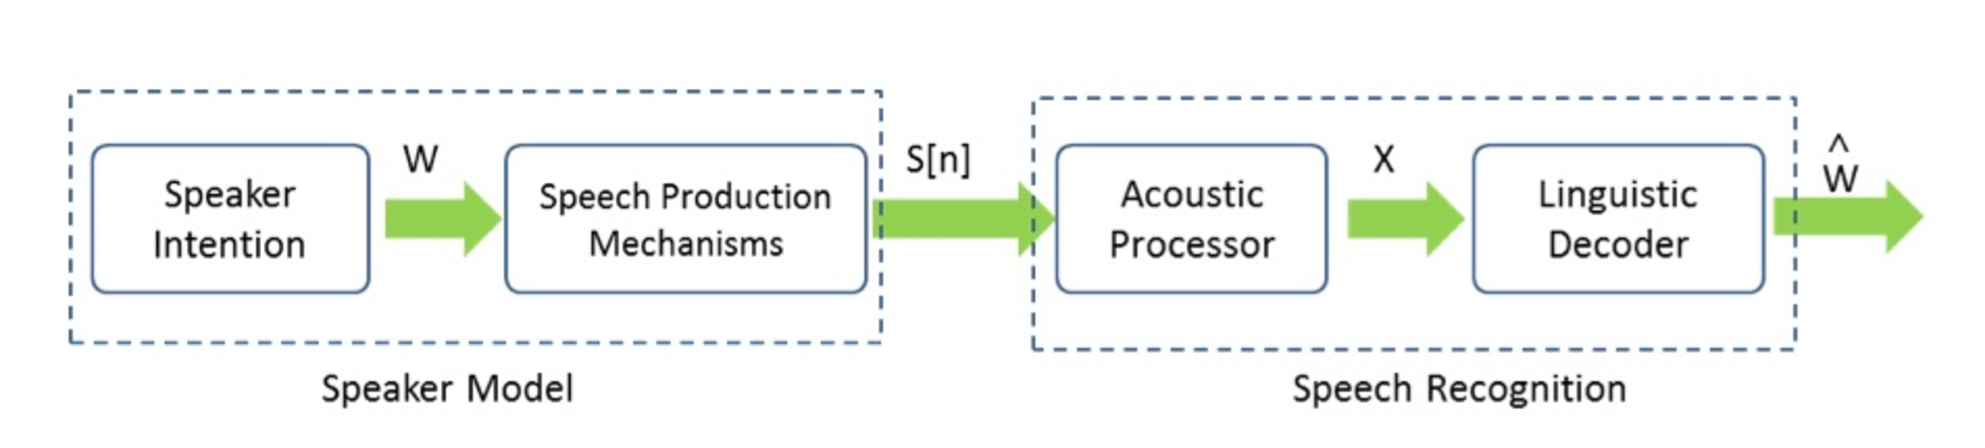
\includegraphics[width=1.0\columnwidth]{images/speechrecognition.pdf}
\caption{Conceptual Model of Speech Production} \label{fig:figure1} 
\end{figure}

A simple conceptual model of human speech production and recognition is shown in Figure (\ref{fig:figure1}). The human speech waveform creation process from the speaker intention is referred as Speaker Model which reflects speaker's accent and choice of words. The Speech Recognizer consists of acoustic processor which analyzes the speech signal and converts it into a set of acoustic (spectral, temporal) features followed by linguistic decoder to estimate the words of spoken sentence.

\section{Speaker Recognition Theory}
The speaker recognition technology is multidisciplinary, which requires hardware based sensors to convert voice in to electrical signals, speech processing module that converters the electrical signals in to digitized data using advanced digital signal processors (DSP). The basic recognition process involves modeling the acoustic data and the natural language to search for patterns. Figure (\ref{fig:figure2}) shows the basic concept of voice recognition.

\begin{figure}
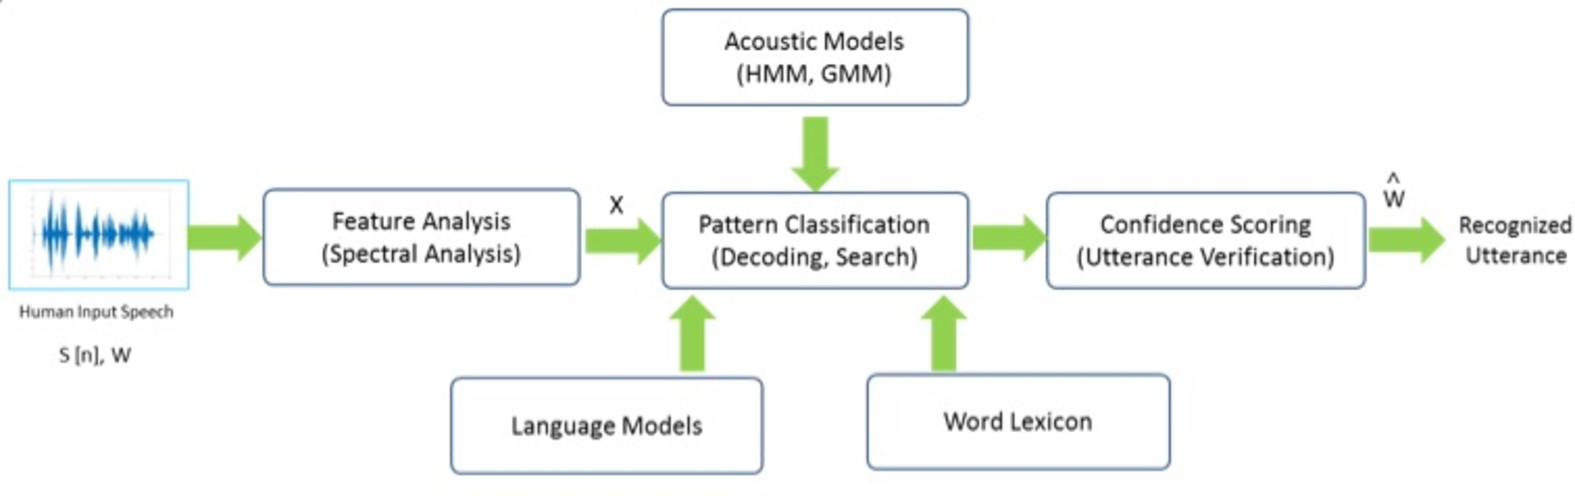
\includegraphics[width=1.0\columnwidth]{images/speakerrecognition.pdf}
\caption{Speaker Recognition Concept}  \label{fig:figure2} 
\end{figure}

As speech is a sound pressure wave, its conversion in to electrical signal and then in to digital signal introduces distortion. As shown in the figure, acoustic front-end requires several signal processing components such as spectral shaping, spectral analysis, spectral modeling, and parametric transformation. These components will condition the signal and establish the spectral measurements and parameters for acoustic modeling.
\par\null\par
Once robust parameterization of speech signal is established, then spectral dynamics or changes of the spectrum with respect to time will be captured. Typically, speaker recognition can be achieved by using differentiation of spectral features, which requires temporal derivatives of the voice spectrum. These temporal derivatives are commonly approximated by differentiating cepstral features using a linear regression. 

\subsection{Feature Analysis}
There are no standard set of features for speech recognition. Instead, various combinations of acoustic, articulatory, and auditory features have been utilized in a range of speech recognition systems \cite{Rabiner2007}. The input human speech signal, s[n], is converted to the series of feature vectors, X = [x1, x2,..., xT], by the feature analysis or spectral analysis module. These feature vectors represent the temporal spectral characteristics of the speech signal in the form of mel frequency cepstrum coefficients.

\subsection{Pattern Classification}
The pattern classification is the process of grouping the patterns, which are sharing the same set of properties \cite{Chandra2014}. The pattern classification involves in computing a match score in speaker recognition system. The term match score refers the similarity of the input feature vectors to some model. Speaker models are built from the feature vectors extracted from the speech signals. Based on the feature extraction a model of the voice is generated and stored in the speaker recognition system. There three major techniques Dynamic Time Warping (DTW), Gaussian Mixture Model (GMM) and Support Vector Machine (SVM) typically used in pattern classification process. 

\subsection{Speaker Acoustic Models}
In the process of recognizing speaker voice, the speaker model will be created and trained with acoustic characteristics of the voice. The typical speaker recognition process involves two specific tasks: verification and identification. In the verification, the goal is to determine from a voice sample if a person is who he or she claims. In the identification, the goal is to determine which one of a group of known voices best matches the input voice sample. In either task the speech can be constrained to be a known phrase (text-dependent) or totally unconstrained (text-independent). The success in both tasks depends on extracting and modeling the speaker-dependent characteristics of the speech signal which can effectively distinguish one talk from another.

A brief description of some of the speaker modeling methods typically used is given below.

\begin{description}

\item[Nearest Neighbor:] In this technique, feature vectors from enrollment (training) speech are retained to represent the speaker. During the verification, the match score is computed as the accumulated distance of each test feature vector to its k nearest neighbors in the speaker's training vectors.

\item[Neural Networks:] These models are trained to discriminate between the speaker being modeled and some alternate speakers.

\item[Hidden Markov Models (HMM):]  The temporal evolution of speech signal features/characteristics and model statistical variations of the features are encoded to provide statistical representation of speaker.

\item[Template Matching:] In this method, the model contains a template with sequence of feature vectors. During the verification a match score is produced by using dynamic time warping (DTW) to align and measure the similarity between test phrase and speaker template.
\end{description}

\section{Natural Language Processing (NLP)} 
NLP is the process of making machines to understand and interpret human languages just the way human beings understands. Speech recognition is the process of analyzing the acoustic data to extract the speech content. In this process speech will be converted in to text as first step. Then, the converted text will be fed to Natural Language Processing (NLP) algorithms for extracting the words and meaning. Machine learning algorithms are used in conjunction with language models to recognize text in natural language processing systems, which may also employ speech models and hardware/software specialized to process and recognize speech. Though human language is ambiguous and unstructured to be interpreted by computers, with the help of NLP, this huge unstructured data can be analyzed for finding the meaning contained inside the data. 

Analyzing language for its meaning is a complex task. Modern speech recognition research began in the late 1950s with the advent of the digital computer \cite{Jacqueline}. The 1960s saw advances in the automatic segmentation of speech into units of linguistic relevance like phonemes, syllables \cite{Peacocke}. And now with advancements in the field of Artificial Intelligence, deep machine learning algorithms have been used in many aspects of speech recognition like Part-of-speech Tagging, Word tokenization, Intent Extraction, phoneme classification, and speaker adaptation. In the context of Speech Recognition, NLP involves five basic steps.
\par\null\par
\textbf{Morphological Analysis:}
     Morphological analysis is the identification, analysis, and description of the structure of a given language's root words,word boundaries, affixes, parts of speech, etc. Non word tokens like punctuation are separated from the words. The term Morpheme means the ``minimal unit of meaning''. For example: In the  word ``unhappiness'' there are three morphemes ``un'', ``happy'', ``ness'' each carrying its own meaning. Morphology treats with the different conjugations of a word and the forms it can take. For example word ``sheep'' can be singular or plural; a verb can have different tenses. 
\par\null\par
\textbf{Syntactic Analysis:}
     Syntactic analysis is the process of analyzing a linear sequence of words in natural language adhering to the rules of a formal grammar of the language. Processing a sentence syntactically includes determining the subject, predicate, verbs, adjectives, pronouns, etc. In this phase, linear sequence of words are converted into hierarchical tree structures that explains how words associate to each other. All most all Syntactic analysis procedures have two components:
     \begin{itemize}
     \item\textit{Grammar:} A declarative expression of syntactic features about the language. It is the specification of the legal structures of a language. It constitutes 3 basic components: Terminal Symbols,Non Terminal Symbols and Rules (productions).
     \item\textit{Parser:} Algorithm that compares the grammar against the input sentences to produce parsed structures called Parse Trees. Parsing can be done in two ways:
      \begin{itemize}
      \item\textit{Top-Down Parsing:} Begin with the start symbol and apply the grammar rules forward until the symbols at the terminals of the tree corresponds to the components of the sentence being parsed \cite{Chakraborty}. 
      \item\textit{Bottom-Up Parsing:} Begin with the sentence to be parsed and apply the grammar rules backward until a single tree whose terminals are the words of the sentence and whose top node is the start symbol has been produced \cite{Chakraborty}. 
      \end{itemize}
     \end{itemize}
\par\null\par
\textbf{Semantic Analysis:}
     Semantic analysis is the process of linking syntactic structures, from the levels of phrases, clauses, sentences and paragraphs to the level of the writing as a whole, to their language-independent meanings. In this phase, the structures created by Syntactic analysis are assigned meanings.
\par\null\par
\textbf{Disclosure Integration:}
     This phase involves resolving of references between sentences. Meaning of one sentence may depend on the meaning earlier sentence. Also meaning of current sentence may influence meaning of following sentences.
\par\null\par
\textbf{Pragmatic Analysis:}
     Pragmatic Analysis is how sentences are used in different situations and how use affects the interpretation of the sentence. Means what was said is reinterpreted as what it actually means. For example: the sentence ``What is the time now?'' should be interpreted as request instead of Question.
\subsection{NLP Techniques}
NLP techniques are broadly categorized into \textit{Rule based (human driven)} and \textit{Statistical based (data driven)}:
\par\null\par
\textbf{Rule based}:
   Rule based (human driven) approach requires huge human effort.Grammars and semantic components are prepared in the form of many carefully handcrafted rules by highly skilled linguists. Rule based approaches takes time, money and trained personnel to make and test the rules. Also rule engineering may not scale very well. To make Rule based approach more accurate, it requires large number of complex hand-written rules which is  much more difficult and laborious task. After certain number of rules, addition of any more rules going to increase the complexity of systems and makes the systems unmanageable.Once there are hundreds of rules, they start interacting in complex ways and becomes difficult while updating or adding any new rules. Rule based approaches have very poor generalization, but for the languages with fewest speakers, rules-based is the best approach since there exist not enough large corpora to go for Statistical approach. The  best  known  parser  with  a  rule base  backbone is the RASP(Robust Accurate Statistical Parsing) system that combines rule-based grammar with a probabilistic parse selection model \cite{Kovar2014}.
\par\null\par
\textbf{Statistical based}:
   Statistical (data driven) approaches treats natural language processing as a \textit{machine learning} problem. They use supervised or unsupervised statistical machine learning algorithms. This method applies learning algorithm to a large body of previously translated text(large data) known as a parallel corpus. Systems based on Statistical approach can be made more accurate by simply supplying more input data.The main advantage of the statistical approach is its language Independence.Provided there are annotated data, the same algorithm can be used for learning rules or models for any language. The statistical approach is significantly leading in terms of accuracy against manually annotated corpora, as well as in overall number of statistical parsers compared to the number of rule-based parsers. Fast, cheap computing hardware, advances in processor speed, random access memory size, secondary storage, and grid computing making Statistical approach as popular choice. One example parser with his approach is MaltParser, a data-driven parser-generator for dependency parsing  that  supports  several  parsing  algorithms  and  learning  algorithms and allows user-defined feature models, consisting of arbitrary combinations of lexical features, part-of-speech features and dependency features. The most significant disadvantage of this approach is the requirement of large amounts of training data in the form of large NL text corpora. 
\par\null\par
Efficient approach is to use both approaches, first use a rule-based model, then use its results as data for the statistical model. 
\subsection{Common usage of Deep learning algorithms in NLP}
\par\null\par
\textbf{Neural Networks:}
  \begin{itemize} 
    \item Part-of-speech Tagging
    \item Word tokenization
    \item Named Entity Recognition
    \item Intent Extraction
  \end{itemize} 
\textbf{Recurrent Neural Networks:}
  \begin{itemize} 
    \item Machine Translation
    \item Question Answering System
    \item Image Captioning
  \end{itemize} 
\textbf{Recursive Neural Networks:}
  \begin{itemize} 
    \item Parsing Sentences
    \item Sentiment Analysis
    \item Relation Classification
  \end{itemize} 
\textbf{Convolutional Neural Networks:}
  \begin{itemize} 
    \item Sentence/Text Classification
    \item Relation Extraction and Classification
    \item Semantic Relation Classification
  \end{itemize} 
\subsection{Speech Recognition Technologies}     
\textbf{Google Cloud Speech API:} Google Cloud Speech API \cite{GoogleSpeech} converts audio to text by applying powerful neural network models in an easy to use API. The API recognizes over 110 languages and supports audio files up to three hours in length. Two basic use cases where Google Cloud Speech apis can be best applied are
  \begin{itemize}
  \item human-computer interaction 
  \item speech analytics on human-to-human interactions.
  \end{itemize} 

\textbf{IBM Watson Speech to Text:} Powerful real-time speech recognition software.Automatically transcribe audio from 7 languages in real-time. Rapidly identify and transcribe what is being discussed, even from lower quality audio, across a variety of audio formats and programming interfaces \cite{IBM}. 

\textbf{Dragon NaturallySpeaking:} Dragon NaturallySpeaking (DNS) \cite{Dragon} is a speech recognition software package developed by Dragon Systems of Newton, Massachusetts. It recognizes and transcribes words at a high speed, and gives flexibility to dictate for any situation. 

\par\null\par
Carnegie Mellon University's Sphinx toolkit, HTK toolkit((free but copyrighted)) and Kaldi tookkits are some good software resources for speech recognition development. 

\section{Confidence Scoring or Speaker Verification}
The confidence scoring process is used to provide a confidence score for each individual word in the recognized string. The scores are produced by extracting confidence features from the computation of the recognition hypothesis and processing the features using accept/reject classifier for word utterance hypothesis. The output of the confidence classifiers can then be incorporated into the parsing mechanism of the language understanding component \cite{Hazen2000}. 

\section{Big Data Context in Speech Analytics}
To get better insight in to customer behavior, satisfaction, and trends information businesses are depending on big data technologies for voice analysis by analyzing large volumes of call data. The use of voice analytics combined with big data technologies will help call centers to improve performance by reducing the call time and repeat calls, providing customer satisfaction information etc.

When applications need continuous recording and processing of large volumes of human speech data for home, industry or public enterprise security/information/entertainment purposes then big data technologies will help meeting the computing and storage demands.  

\section{Integrated Speech and Voice Recognition Applications}
Voice biometrics, customer service, truth detection, and personal voice assistant are some of the applications currently being used by the industry with speech recognition and analytics as key underlying technologies. Voice recognition technology has been in use by security systems with voice activated locks, law enforcement and criminology for truth detection. 

In the customer service industry, speech analytics is playing key role to get complete insight in to customer behaviors and interests. Customers will interact with service providers using multiple channels such as email, social media, SMS, phone call, and in-person etc. The technology advancements are creating even more channels or options to interact with customers and service providers.  However, with speech analytics systems the business can get more hidden insights for improving the customer satisfaction and loyalty. The capabilities such as phonetic-indexing, speech-to-text transcripts, speaker separation, emotion detection, and hot topics etc. are already in use by several businesses to improve their customer service performance.

The integrated speech and voice recognition will take the solution use cases one step beyond the current applications use and help improving the business performances. For example, systems will recognize returning customers with voice recognition technology and engage them with personalized interests/conversations. 

\section{Conclusion}
 The voice, speech recognition technologies and NLP combined with big data technologies can be used in solving much complex problems than the current applications. Potential applications include personalized customer services, personal voice assists, and public information desks etc. 
 
 An attempt has been made to explain speech and speaker recognition concepts along with big data technology use in the applications. Then, some of the typical speaker acoustic models and pattern classification and platter recognition methods have been listed. There are several companies and entrepreneurs researching to create better Natural Language Processing (NLP) solutions and teach computers how to better understand human communication. Some of the unsolved technologies such as cross language translators and accurate speaker recognition are still in research, which when solved can unleash the great potential across the world.

\begin{acks}

  The authors would like to thank professor Gregor von Laszewski and his team for providing \textit{LaTex} templates and assistance with the \textit{JabRef} tool to organize references.


\end{acks}

\bibliographystyle{ACM-Reference-Format}
\bibliography{report} 
\newpage
\appendix
\section{Work Breakdown}
\subsection{HID 333:Anil Ravi}
\begin{itemize}
  \item Identified Paper2 topic.
  \item Created Paper2 draft sections.
  \item Finalized speech recognition theory.
  \item Reviewed all sections of the paper.
\end{itemize}
\subsection{HID 337:Ashok Reddy Singam}
\begin{itemize}
  \item Worked on NLP and its subsections.
  \item Editing Latex template using ShareLatex online tool.
  \item Managed JabRef entries.
  \item Reviewed the draft paper.
\end{itemize}



\end{document}
